\documentclass[12pt]{article}

\title{CSC 420 - Assignment 2}
\author{ Group 3 \\
        Robert Krency, kre1188@calu.edu}
\date{\today}

\usepackage{tikz}
\usepackage{amsmath}
\usepackage{graphicx}
\usepackage{tabularx}
\usepackage{multicol}
\usepackage{algpseudocode}
\usepackage{algorithm}
\usepackage{setspace}

% Geometry 
\usepackage{geometry}
\geometry{letterpaper, left=20mm, top=20mm, right=20mm, bottom=20mm}

\onehalfspacing

% Add vertical spacing to tables
\renewcommand{\arraystretch}{1.4}

% Macros
\newcommand{\definition}[1]{\underline{\textbf{#1}}}

\newenvironment{rcases}
  {\left.\begin{aligned}}
  {\end{aligned}\right\rbrace}

% Begin Document
\begin{document}

\maketitle

\vspace{1cm}

\section{Question 1}

Determine the order of nodes visited in the graph with each of the following algorithms:

\begin{enumerate}
    \item Breadth-First Search
    \begin{enumerate}
        \item 1, 2, 3, 4, 5, 6, 7, 8, 9, 10, 11, 12
    \end{enumerate}

    \item Depth Limited Search (limit: 3)
    \begin{enumerate}
        \item 1, 2, 4, 8, 9, 5, 10, 11, 3, 6, 12
    \end{enumerate}

    \item Iterative Deepening Search
    \begin{enumerate}
        \item Limit 1 $\to$ 1, 2, 3
        \item Limit 2 $\to$ 1, 2, 4, 5, 3, 6, 7
        \item Limit 3 $\to$ 1, 2, 4, 8, 9, 5, 10, 11, 3, 6, 7
    \end{enumerate}

\end{enumerate}


\pagebreak
\section{Question 2}

\subsection{Problem Formulation}

\begin{description}
    \item[Initial State:] The Robot is at (1,1), 10 objects are available for pickup, 10 destinations are open for drop off.
    \item[Goal State:] The Robot is at (1,1) and all objects are placed in a destination.
    \item[Transition:] Go(row\#, col\#) moves the robot to the grid cell (row\#, col\#) 
    \item[Action Cost:] The amount of grid spaces needed to move from current to destination.  
\end{description}

In this case, each state would represent the action of moving to an Object and then moving it to a Destination.
The robot, in all cases, would also require a concluding action of returning to the start position.

As we generate each node, we would account for four values:

\begin{enumerate}
    \item Total Distance Traveled
    \item Distance between the Robot and the Object
    \item Distance between the Object and its Destination
    \item The heuristic value
\end{enumerate}

The proposed heuristic value would be the sum of two values:

\begin{enumerate}
    \item The sum of the distances between remaining objects and their closest open destination
    \item The distance between the destination and the start position
\end{enumerate}

\subsection{Search Algorithm Usage}

I would recommend usage of the A* algorithm in this case.
If we consider that moving to an object and then moving that object to a destination to be a State, 
then the maximum amount of States that could be visited with $n$ nodes would be $O((n!)^2)$.


\pagebreak

\section{Question 3}

\subsection{Expand Dobreta}

\begin{center}
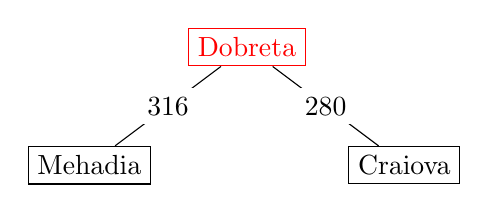
\begin{tikzpicture}
    
    \node [red] [draw] {Dobreta} [sibling distance = 4cm]
        child {node [draw] {Mehadia} edge from parent node [draw=none,fill=white] {$316$}}
        child {node [draw] {Craiova} edge from parent node [draw=none,fill=white] {$280$}};

\end{tikzpicture}
\end{center}

\subsection{Expand Craiova}

\begin{center}
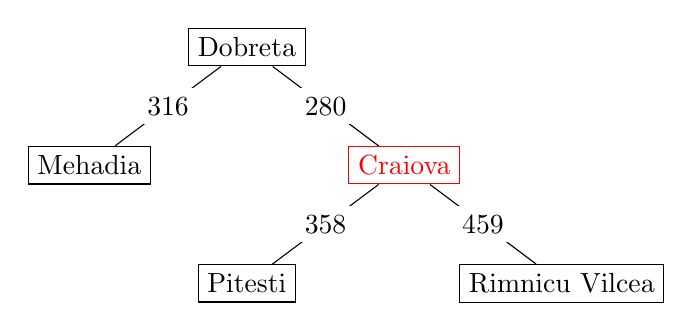
\begin{tikzpicture}
    
    \node [draw] {Dobreta} [sibling distance = 4cm]
        child {node [draw] {Mehadia} edge from parent node [draw=none,fill=white] {$316$}}
        child {node [red] [draw] {Craiova}
            child {node [draw] {Pitesti} edge from parent node [draw=none,fill=white] {$358$}}
            child {node [draw] {Rimnicu Vilcea} edge from parent node [draw=none,fill=white] {$459$}}
            edge from parent node [draw=none,fill=white] {$280$}}

        ;

\end{tikzpicture}
\end{center}

\subsection{Expand Mehadia}

\begin{center}
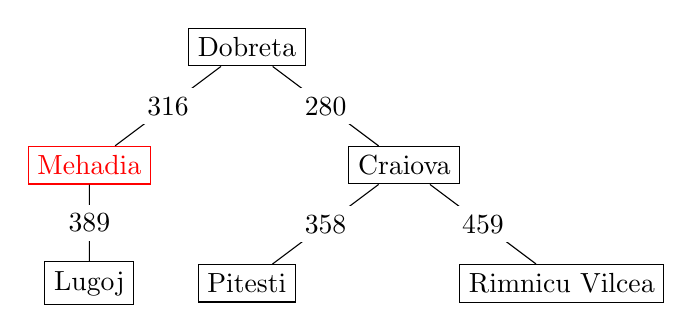
\begin{tikzpicture}
    
    \node [draw] {Dobreta} [sibling distance = 4cm]
        child {node [red] [draw] {Mehadia}
            child {node [draw] {Lugoj} edge from parent node [draw=none,fill=white] {$389$}}
            edge from parent node [draw=none,fill=white] {$316$}
        }
        child {node [draw] {Craiova}
            child {node [draw] {Pitesti} edge from parent node [draw=none,fill=white] {$358$}}
            child {node [draw] {Rimnicu Vilcea} edge from parent node [draw=none,fill=white] {$459$}}
            edge from parent node [draw=none,fill=white] {$280$}
        }

        ;

\end{tikzpicture}
\end{center}

\subsection{Expand Pitesti}

\begin{center}
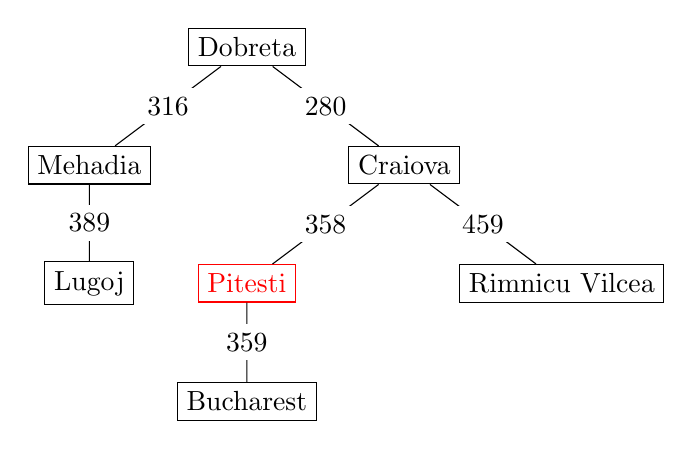
\begin{tikzpicture}
    
    \node [draw] {Dobreta} [sibling distance = 4cm]
        child {node [draw] {Mehadia}
            child {node [draw] {Lugoj} edge from parent node [draw=none,fill=white] {$389$}}
            edge from parent node [draw=none,fill=white] {$316$}
        }
        child {node [draw] {Craiova}
            child {node [red] [draw] {Pitesti}
                child {node [draw] {Bucharest} edge from parent node [draw=none,fill=white] {$359$}}
                edge from parent node [draw=none,fill=white] {$358$}
            }
            child {node [draw] {Rimnicu Vilcea} edge from parent node [draw=none,fill=white] {$459$}}
            edge from parent node [draw=none,fill=white] {$280$}
        }

        ;

\end{tikzpicture}
\end{center}

\subsection{Expand Bucharest}

\begin{center}
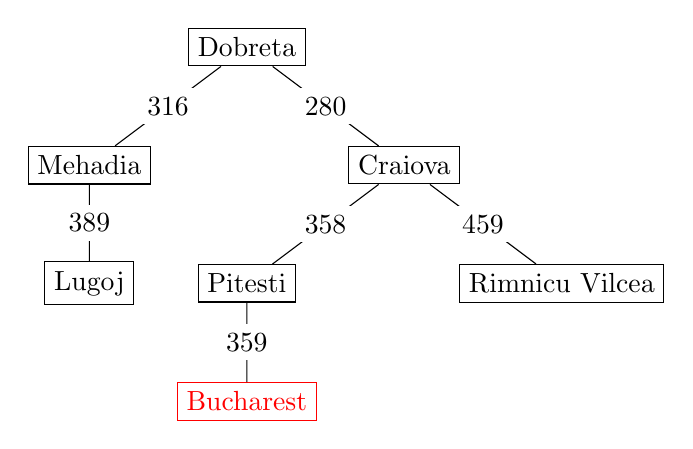
\begin{tikzpicture}
    
    \node [draw] {Dobreta} [sibling distance = 4cm]
        child {node [draw] {Mehadia}
            child {node [draw] {Lugoj} edge from parent node [draw=none,fill=white] {$389$}}
            edge from parent node [draw=none,fill=white] {$316$}
        }
        child {node [draw] {Craiova}
            child {node [draw] {Pitesti}
                child {node [red] [draw] {Bucharest} edge from parent node [draw=none,fill=white] {$359$}}
                edge from parent node [draw=none,fill=white] {$358$}
            }
            child {node [draw] {Rimnicu Vilcea} edge from parent node [draw=none,fill=white] {$459$}}
            edge from parent node [draw=none,fill=white] {$280$}
        }

        ;

\end{tikzpicture}
\end{center}

Search ends here, as the expansion candidate is the goal.


\end{document}
